
%(BEGIN_QUESTION)
% Copyright 2010, Tony R. Kuphaldt, released under the Creative Commons Attribution License (v 1.0)
% This means you may do almost anything with this work of mine, so long as you give me proper credit

Suppose you needed to simulate an RTD to the input of a temperature transmitter, using a $3 \over 4$-turn potentiometer:

$$\includegraphics[width=15.5cm]{i00590x01.eps}$$

Sketch the necessary connecting wires so that the simulated RTD signal to the transmitter increases as the potentiometer's shaft is rotated {\it clockwise}, and so that the multimeter registers the transmitter's 4-20 mA signal (using the batteries as a 24 VDC loop power supply) as a positive numerical value.

\vskip 10pt

Note the internal construction of a typical $3 \over 4$-turn potentiometer, as shown in this illustration:

$$
\includegraphics[width=5.5cm]{i00590x03.eps}$$

\vfil 

\underbar{file i00590}
\eject
%(END_QUESTION)





%(BEGIN_ANSWER)

This is a graded question -- no answers or hints given!

%(END_ANSWER)





%(BEGIN_NOTES)

According to the symbols drawn near the transmitter's RTD connection terminals, this is a 3-wire RTD transmitter.  Thus, we {\it must} use a 3-wire cable to connect the transmitter to the RTD in order to avoid measurement errors.

\vskip 10pt

First, we identify which two terminals on the potentiometer will increase resistance as we turn the knob clockwise.  From an inspection of the pot's internal construction, we can see these will be the middle and right terminals: as the wiper rotates clockwise, it approaches the left terminal and gets farther away from the right terminal.

\vskip 10pt

Next, we connect these two terminals on the pot to the two terminals on the transmitter which need to see the main RTD resistance (i.e. the middle and bottom terminals on the transmitter).  After that, we need to connect our third and last wire from the top transmitter terminal to a point on the pot that is common with the wire connecting to the transmitter's middle terminal.  These connections are absolutely essential to get right.

\vskip 10pt

As for the 4-20 mA loop wiring, any series connection that lets the batteries aid each other, and connects both the meter and transmitter as loads, is correct.

\vskip 10pt

One solution is shown here:

$$\includegraphics[width=15.5cm]{i00590x02.eps}$$

%INDEX% Measurement, temperature: RTD resistance calibration

%(END_NOTES)

